\section{Extensibility, Inspectability and Expressiveness}
\label{sec:features}

The features in Section~\ref{sec:motivation} form the basis of \dsl{}.
To provide support for additional features present in other animation libraries,
we design \dsl{} to be extensibile and
inspectable. This means that \dsl{} can be extended with new
operations and information can be derived from inspecting specified animations.
To support arbitrary expressiveness in combination with those
features, we also emphasize the possibility to extend \dsl{} with new
combinators.

\subsection{Extensibility}
\label{sec:customop}

The \hs{linearTo} operation and the \hs{sequential} and \hs{parallel} combinators form the basis for expressing a variety of animations. However, there are situations which require other primitives to express desired animations. For example, GSAP provides a primitive to morph one shape into another.

An example in the to-do list app is the \hs{checkIcon} animation, part of the \hs{markAsDone} animation, where we want to set the color of the checkmark to a new value. We define a custom \hs{set} operation and embed it inside a \dsl{} animation. In this animation we use Haskell's \hs{do}-notation to specify sequential animations.

\begin{spec}
checkIcon = do ...; set (checkmark . color) green; ...
\end{spec}

%\begin{figure}[h]
%\centering
%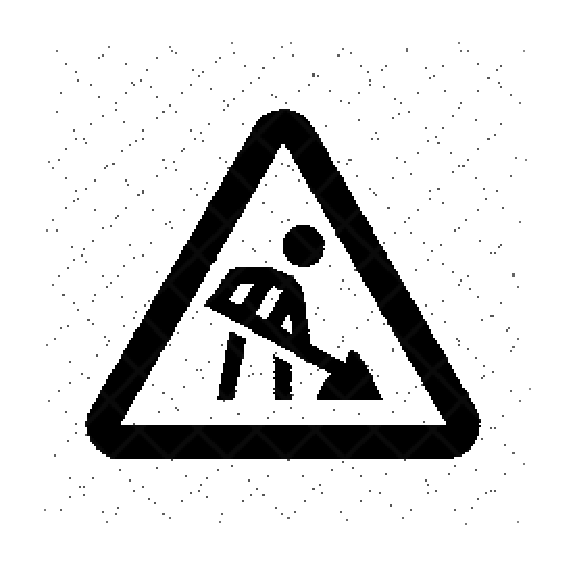
\includegraphics[width=\figscale\textwidth]{pictures/todo}
%\caption{The \hs{checkIcon} animation.}
%\label{fig:}
%\end{figure}

\subsection{Inspectability}

\dsl{} is inspectable, meaning that we can derive properties of expressed computations by \emph{inspecting them rather than running them}. For example, if we want to know the duration of \hs{menuIntro} without actually running it and keeping track of the time. We can do this by using a predefined \hs{duration} function, which calculates the duration by inspecting the animation. This gives a duration of \hs{0.5} seconds, which is indeed the duration of two \hs{0.5} second animations in parallel.

\begin{spec}
menuIntroDuration = duration menuIntro -- = 0.5
\end{spec}

Of course, it is not possible to inspect every animation. In the following situation we have a custom operation \hs{get}, the dual of \hs{set} in the previous section, returning a \hs{Float}. If the result of this value is used as the duration parameter of an animation, then we cannot know upfront how long this animation will last. Requesting to calculate the duration of such an animation results in a type error.

\begin{spec}
complicatedAnim = do v <- get; linearTo lens (For v) (To 10)
complicatedAnimDuration = duration complicatedAnim -- type error
\end{spec}

Calculating a duration is a stepping stone towards other interesting features. One such example is sequentially composing animations with a relative offset. For example, to compose a first animation \hs{anim1} with a second animation \hs{anim2} which starts 0.5 seconds \emph{before} the end of \hs{anim1}.

\begin{spec}
relSeqAnim = relSequential anim1 anim2 (-0.5)
\end{spec}

\subsection{Expressiveness}
\label{sec:customcomb}

In monadic DSLs the \hs{>>=} and \hs{return} combinators provide the needed expressivity. When creating inspectable animations, \hs{>>=} is a liability since it has limited inspectability. \dsl{} supports extension with custom control flow combinators.

The \hs{onlyDone} animation shows all \emph{done} items while
hiding all \emph{to-do} items. This could be implemented by first
showing all items with the \hs{showAll} animation, since an item might have
been hidden by a previous action, and then hiding all to-do items with the
\hs{hideToDo} animation. The definition is given below, while the definitions
of \hs{showAll} and \hs{hideToDo} are omitted for brevity.

\begin{spec}
onlyDoneNaive = do showAll; hideToDo
\end{spec}

However, the intended animation is to only show done items when any were hidden.
So instead we first check the amount and based on that we play the naive version of \hs{onlyDone},
otherwise we just hide the not done items.

\begin{spec}
onlyDone = do
  cond <- doneItemsGt0    -- check if more than 0 'done' items
  if cond then onlyDoneNaive else hideToDo
\end{spec}

However, this formulation uses monadic features and is thus not inspectable.
To make it inspectable, we utilize a custom combinator \hs{ifThenElse}.
We revisit this example in more detail in Section~\ref{sec:interaction}.

\begin{spec}
onlyDone = ifThenElse doneItemsGt0 onlyDoneNaive hideToDo
\end{spec}

For this new combinator, we can define custom ways to inspect it. Since each
branch might have a different duration, we do not choose to extract the
duration but rather the \emph{maximum} duration of the animation.

\begin{spec}
onlyDoneMaxDuration = maxDuration onlyDone -- = 1
\end{spec}

Sections~\ref{sec:motivation} and \ref{sec:features} gave a look and feel of the
features of \dsl{}. In the following sections, we delve deeper into the
internals of the implementation.
